\section{Lagrange Interpolation}
\label{sec:math_lagrange}

We spend some time discussing \gls{lagrange interpolation}.

\subsection{Why do we care about interpolation?}

Within cryptography, \emph{\gls{lagrange interpolation}}
over \glspl{finite field}
is used in secret sharing protocols and \gls{distributed key generation}.
More generally, interpolation is useful because
it attempts to approximate a complex function with a simpler polynomial.

We will start by looking at interpolation over real data.
After working through examples, we will transition
to interpolation over \glspl{finite field} as this is our primary focus.

\subsection{Lagrange Interpolation over the Reals}

Given a set of data points $\braces{\parens{x_{k},y_{k}}}_{k=1}^{n}$
with $\braces{x_{k}}_{k=1}^{n}$ distinct,
we want to find the interpolating polynomial of minimal degree
which agrees with the data.
That is, we want a polynomial $p$ of at most degree $n-1$ such that

\begin{equation}
    p(x_{k}) = y_{k}, \quad k\in\braces{1,\cdots,n}.
\end{equation}

We now proceed to construct such a polynomial.
To do this, we set

\begin{align}
    L(x) &\mathDef{} \sum_{k=1}^{n} y_{k}\ell_{k}(x) \nonumber\\
    \ell_{k}(x) &\mathDef{}
        \prod_{\substack{1\le j \le n \\ j\ne k}} \frac{x-x_{j}}{x_{k}-x_{j}}
            \nonumber\\
        &=
        \frac{x-x_{1}}{x_{k}-x_{1}}\cdot
        \frac{x-x_{2}}{x_{k}-x_{2}}\cdots
        \frac{x-x_{k-1}}{x_{k}-x_{k-1}}\cdot
        \frac{x-x_{k+1}}{x_{k}-x_{k+1}}\cdots
        \frac{x-x_{n}}{x_{k}-x_{n}}.
    \label{eq:math_lagrange_def}
\end{align}

\noindent
We note that $\ell_{k}$ is a polynomial of degree $n-1$;
this implies that $L$ is a polynomial of degree at most $n-1$.
We note that

\begin{align}
    \ell_{k}(x_{j}) &=
        \begin{cases} 1, \quad k = j \\ 0, \quad k\ne j \end{cases}
            \nonumber\\
        &= \del_{kj}.
\end{align}

\noindent
Here, $\del_{kj}$ is the Kronecker delta.
It follows that 

\begin{align}
    L(x_{j}) &= \sum_{k=1}^{n}y_{k}\ell_{k}(x_{j}) \nonumber\\
        &= \sum_{k=1}^{n} y_{k}\del_{kj} \nonumber\\
        &= y_{j}.
\end{align}

\noindent
Thus, this is the interpolating polynomial which agrees
with the data.
Furthermore, the degree of the polynomial is at most $n-1$.
Such polynomials are unique.

\subsection{Examples of Lagrange Interpolation over the Reals}

\begin{example}
\label{example:math_lagrange_reals_1}
\exampleCodeReference{examples/math\_review/lagrange\_reals\_1.py}

We begin by interpolating the data
$\braces{\parens{1,2},\parens{4,1},\parens{7,8}}$.
See the data in Figure~\ref{fig:lagrange_points_1}.

\begin{figure}[t]
\centering
    \begin{subfigure}[t]{0.45\textwidth}
    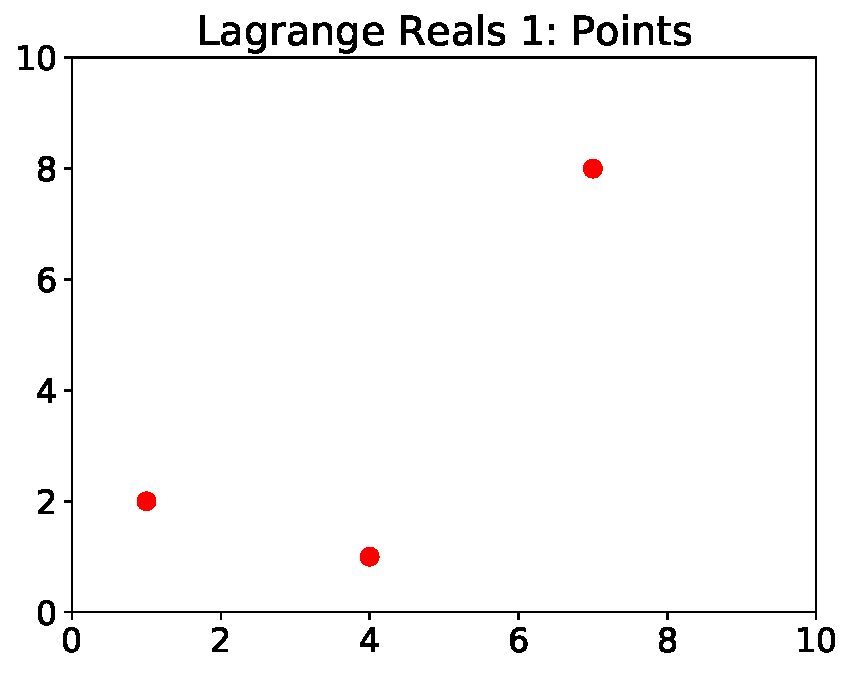
\includegraphics[width=\textwidth]{plots/lagrange/lagrange_reals_points_1.pdf}
    \caption{Lagrange interpolation data points}
    \label{fig:lagrange_points_1}
    \end{subfigure}
    \begin{subfigure}[t]{0.45\textwidth}
    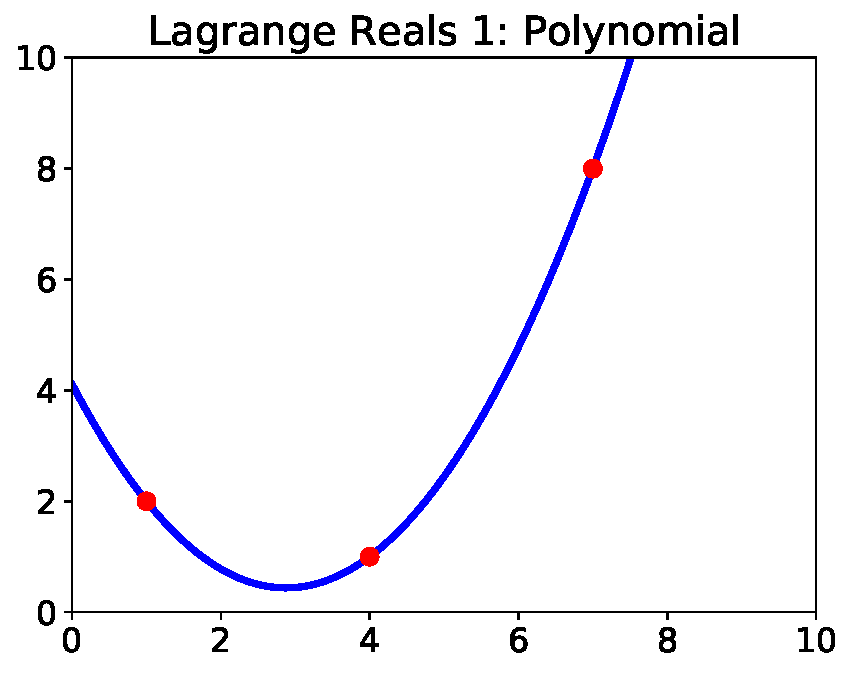
\includegraphics[width=\textwidth]{plots/lagrange/lagrange_reals_poly_1.pdf}
    \caption{Lagrange interpolation polynomial}
    \label{fig:lagrange_poly_1}
    \end{subfigure}
    \caption[Data points and Lagrange Interpolation over the reals 1]{Here
        are data points and Lagrange interpolating polynomial
        for Example~\ref{example:math_lagrange_reals_1}.}
\end{figure}



We start by computing the $\ell_{k}$ polynomials:

\begin{align}
    \ell_{1}(x) &= \frac{x-4}{1-4}\cdot\frac{x-7}{1-7}
        \nonumber\\
    \ell_{2}(x) &= \frac{x-1}{4-1}\cdot\frac{x-7}{4-7}
        \nonumber\\
    \ell_{3}(x) &= \frac{x-1}{7-1}\cdot\frac{x-4}{7-4}.
\end{align}

\noindent
In this case, we have the interpolating polynomial

\begin{equation}
    L(x) = 2\cdot\frac{x-4}{1-4}\cdot\frac{x-7}{1-7}
        + 1\cdot\frac{x-1}{4-1}\cdot\frac{x-7}{4-7}
        + 8\cdot\frac{x-1}{7-1}\cdot\frac{x-4}{7-4}.
\end{equation}

\noindent
This may be reduced to

\begin{equation}
    L(x) = \frac{1}{9}\brackets{4x^{2} - 23x + 37}.
\end{equation}

\noindent
The data points with this polynomial can be found in
Figure~\ref{fig:lagrange_poly_1}.
We see that

\begin{align}
    L(1) &= 2 \nonumber\\
    L(4) &= 1 \nonumber\\
    L(7) &= 8.
\end{align}
\end{example}

\begin{example}
\label{example:math_lagrange_reals_2}
\exampleCodeReference{examples/math\_review/lagrange\_reals\_2.py}

We interpolate the data
$\braces{\parens{1,2},\parens{4,1},\parens{5,1},\parens{7,8}}$;
this is the same data from the previous example with the additional
point $\parens{5,1}$.
See the data in Figure~\ref{fig:lagrange_points_2}.

\begin{figure}[t]
\centering
    \begin{subfigure}[t]{0.45\textwidth}
    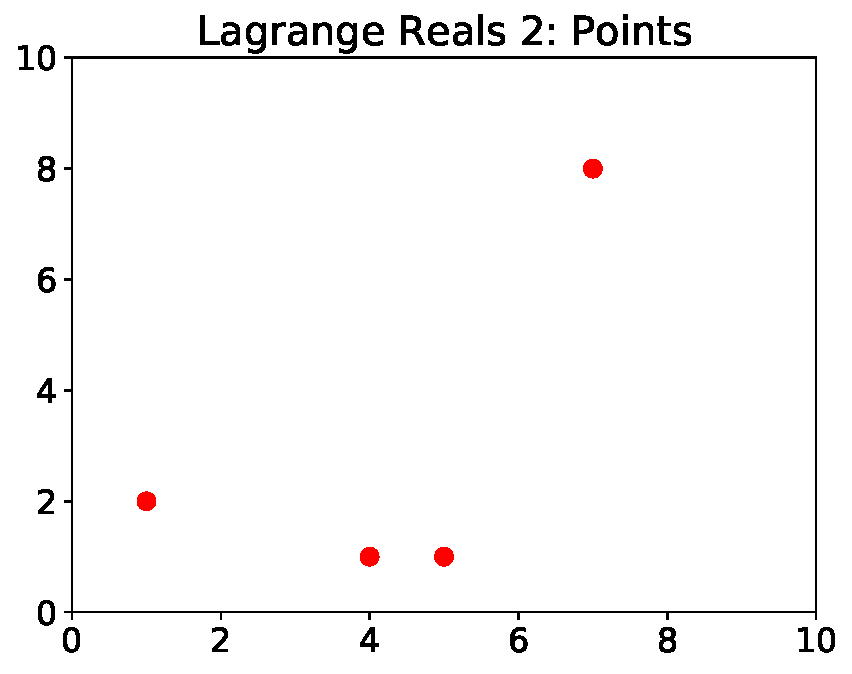
\includegraphics[width=\textwidth]{plots/lagrange/lagrange_reals_points_2.pdf}
    \caption{Lagrange interpolation data points}
    \label{fig:lagrange_points_2}
    \end{subfigure}
    \begin{subfigure}[t]{0.45\textwidth}
    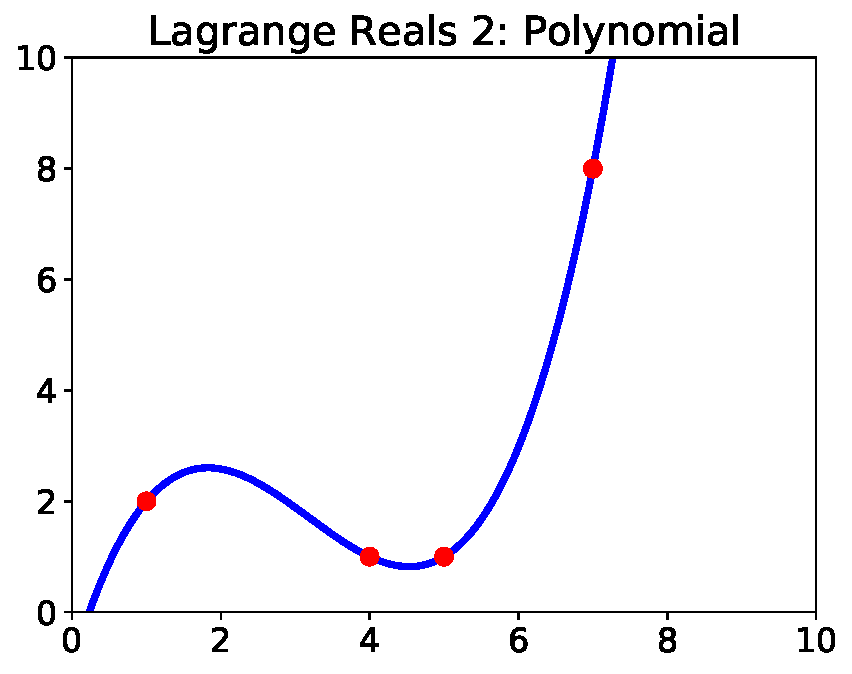
\includegraphics[width=\textwidth]{plots/lagrange/lagrange_reals_poly_2.pdf}
    \caption{Lagrange interpolation polynomial}
    \label{fig:lagrange_poly_2}
    \end{subfigure}
    \caption[Data points and Lagrange Interpolation over the reals 2]{Here
        are data points and Lagrange interpolating polynomial
        for Example~\ref{example:math_lagrange_reals_2}.}
\end{figure}



We again compute the $\ell_{k}$ polynomials:

\begin{align}
    \ell_{1}(x) &= \frac{x-4}{1-4}\cdot\frac{x-5}{1-5}\cdot\frac{x-7}{1-7}
        \nonumber\\
    \ell_{2}(x) &= \frac{x-1}{4-1}\cdot\frac{x-5}{4-5}\cdot\frac{x-7}{4-7}
        \nonumber\\
    \ell_{3}(x) &= \frac{x-1}{5-1}\cdot\frac{x-4}{5-4}\cdot\frac{x-7}{5-7}
        \nonumber\\
    \ell_{4}(x) &= \frac{x-1}{7-1}\cdot\frac{x-4}{7-4}\cdot\frac{x-5}{7-5}.
\end{align}

\noindent
The resulting Lagrange interpolation polynomial is

\begin{equation}
    L(x) = \frac{1}{72}\brackets{13x^{3} - 124x^{2} + 323x - 68}.
\end{equation}

\noindent
The data points with this polynomial can be found in
Figure~\ref{fig:lagrange_poly_2}.
\end{example}

\subsection{Problems with Lagrange Interpolation over the Reals}

We note that using \gls{lagrange interpolation} can lead to problems
when attempting to approximate certain types of \glspl{function} (data).
In particular, even with smooth functions
(functions with infinitely many derivatives),
it is possible that the polynomial approximation given by
\gls{lagrange interpolation} does not converge to the underlying function.
An example of this is shown in Figure~\ref{fig:math_lagrange_runge};
this is called \emph{Runge's Phenomenon}.

\begin{figure}[t]
\centering
    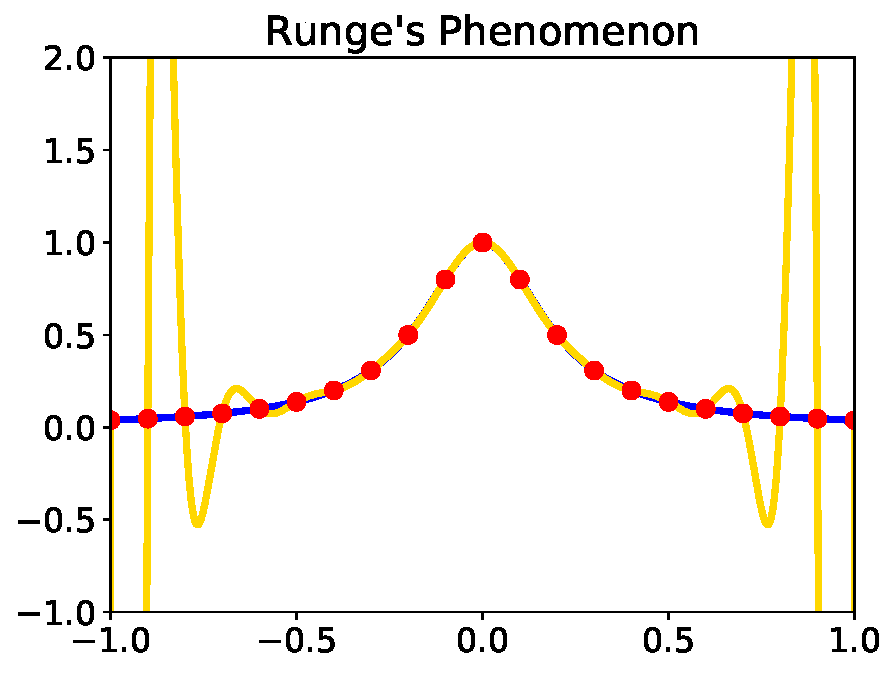
\includegraphics[width=10cm]{plots/lagrange/lagrange_runge.pdf}
    \caption[Plot of Runge's Phenomenon]{Here
        is an example of Runge's phenomenon.
        Even though the polynomial approximation of the \gls{function}
        $f(x) = \brackets{1+25x^{2}}^{-1}$
        is accurate close to $0$, the approximation is very poor
        near $1$ and $-1$.}
    \label{fig:math_lagrange_runge}
\end{figure}


There are mathematical reasons which can explain this,
but \emph{none} of those difficulties matter to us
because we are not particularly interested in interpolating
\glspl{function} over $\R$.
Rather, we are interested in interpolating polynomials over
\glspl{finite field}.

\subsection{Lagrange Interpolation over Finite Fields}

We are particularly interested in performing \gls{lagrange interpolation}
over \glspl{finite field}.
This will be used in secret sharing protocols.

There is effectively no difference between interpolation
over $\R$ and interpolation over $\F_{p}$.
This is because all of the operations in $\R$ directly translate
into the equivalent operations in $\F_{p}$.

\subsection{Examples of Lagrange Interpolation over Finite Fields}

We use the same examples as before except that now we use
the \gls{finite field} $\F_{73}$.



\begin{example}
\label{example:math_lagrange_finite_1}
\exampleCodeReference{examples/math\_review/lagrange\_finite\_1.py}

We begin by interpolating the data
$\braces{\parens{1,2},\parens{4,1},\parens{7,8}}$ as before
in Example~\ref{example:math_lagrange_reals_1};
in this case, we are interpolating over $\F_{73}$.
See the data in Figure~\ref{fig:lagrange_finite_points_1}.

\begin{figure}[t]
\centering
    \begin{subfigure}[t]{0.45\textwidth}
    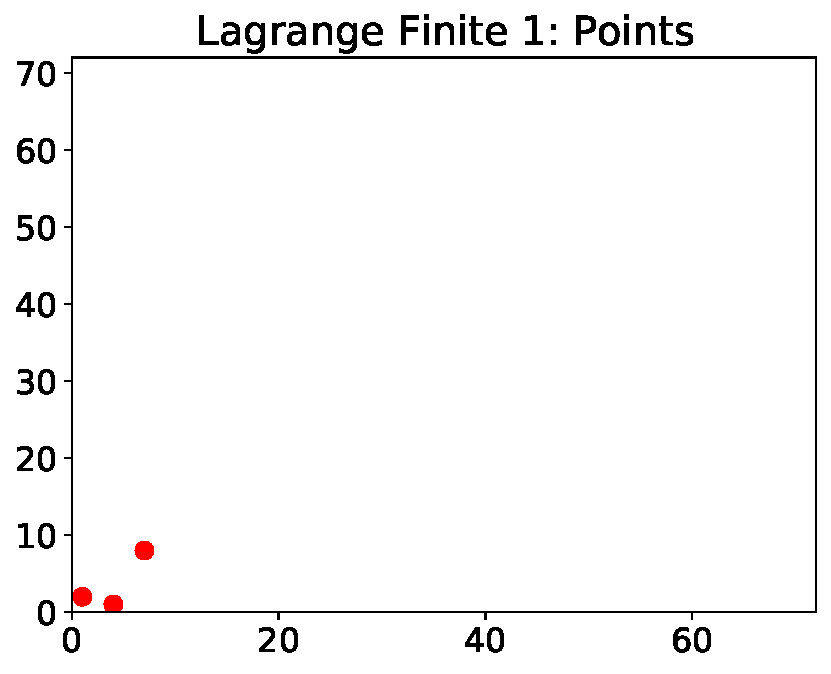
\includegraphics[width=\textwidth]{plots/lagrange/lagrange_finite_points_1.pdf}
    \caption{Lagrange interpolation data points}
    \label{fig:lagrange_finite_points_1}
    \end{subfigure}
    \begin{subfigure}[t]{0.45\textwidth}
    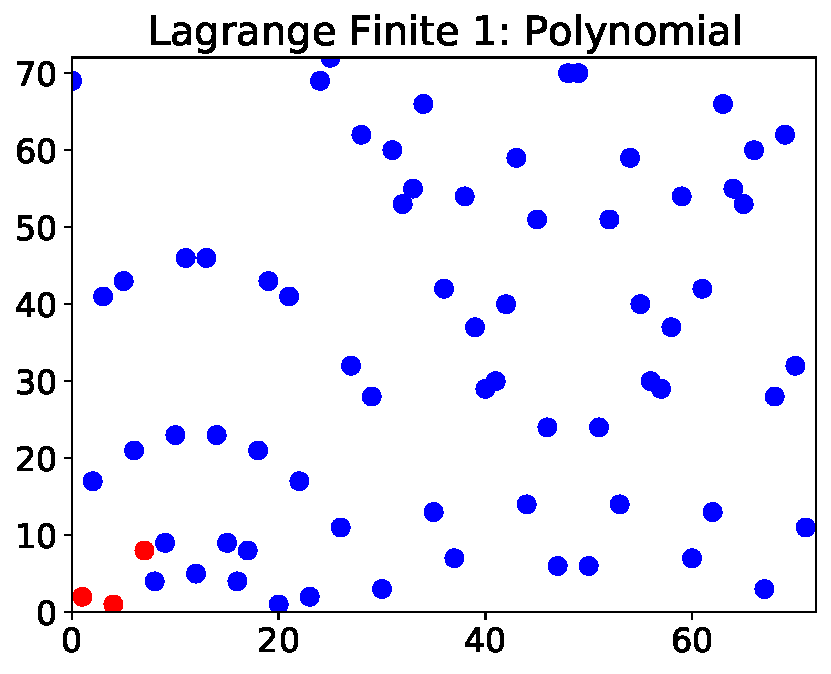
\includegraphics[width=\textwidth]{plots/lagrange/lagrange_finite_poly_1.pdf}
    \caption{Lagrange interpolation polynomial}
    \label{fig:lagrange_finite_poly_1}
    \end{subfigure}
    \caption[Data points and Lagrange Interpolation over finite fields 1]{Here
        are data points and Lagrange interpolating polynomial
        for Example~\ref{example:math_lagrange_finite_1}.
        This example uses the \gls{finite field} $\F_{73}$.}
\end{figure}



In this case, we have the interpolating polynomial

\begin{equation}
    L(x) = 41x^{2} + 38x + 69.
\end{equation}

\noindent
The data points with this polynomial can be found in
Figure~\ref{fig:lagrange_finite_poly_1}.
We see that

\begin{align}
    L(1) &= 2 \nonumber\\
    L(4) &= 1 \nonumber\\
    L(7) &= 8.
\end{align}
\end{example}

\begin{example}
\label{example:math_lagrange_finite_2}
\exampleCodeReference{examples/math\_review/lagrange\_finite\_2.py}

We interpolate the data
$\braces{\parens{1,2},\parens{4,1},\parens{5,1},\parens{7,8}}$ as
in Example~\ref{example:math_lagrange_reals_2};
in this case, we are interpolating over $\F_{73}$.
See the data in Figure~\ref{fig:lagrange_finite_points_2}.

\begin{figure}[t]
\centering
    \begin{subfigure}[t]{0.45\textwidth}
    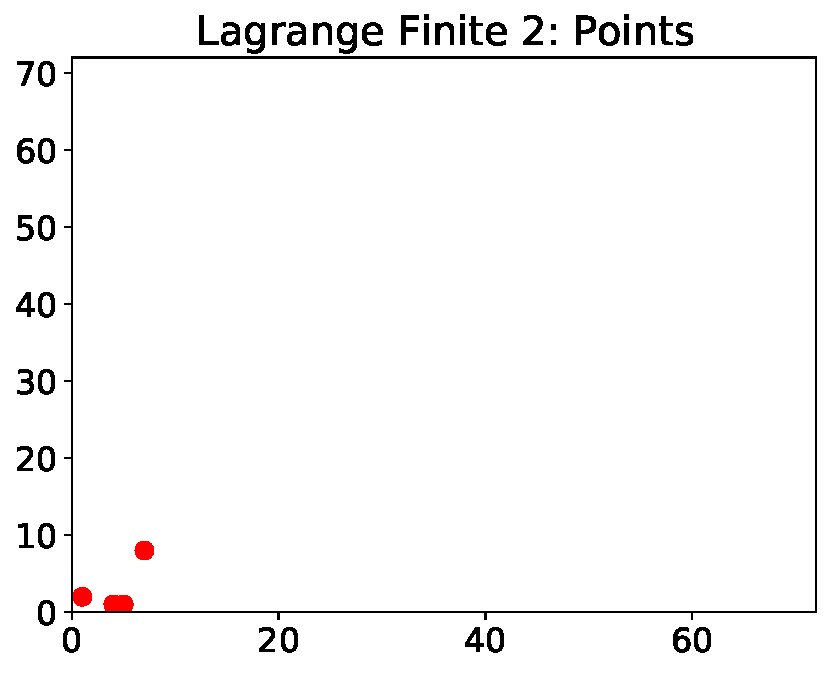
\includegraphics[width=\textwidth]{plots/lagrange/lagrange_finite_points_2.pdf}
    \caption{Lagrange interpolation data points}
    \label{fig:lagrange_finite_points_2}
    \end{subfigure}
    \begin{subfigure}[t]{0.45\textwidth}
    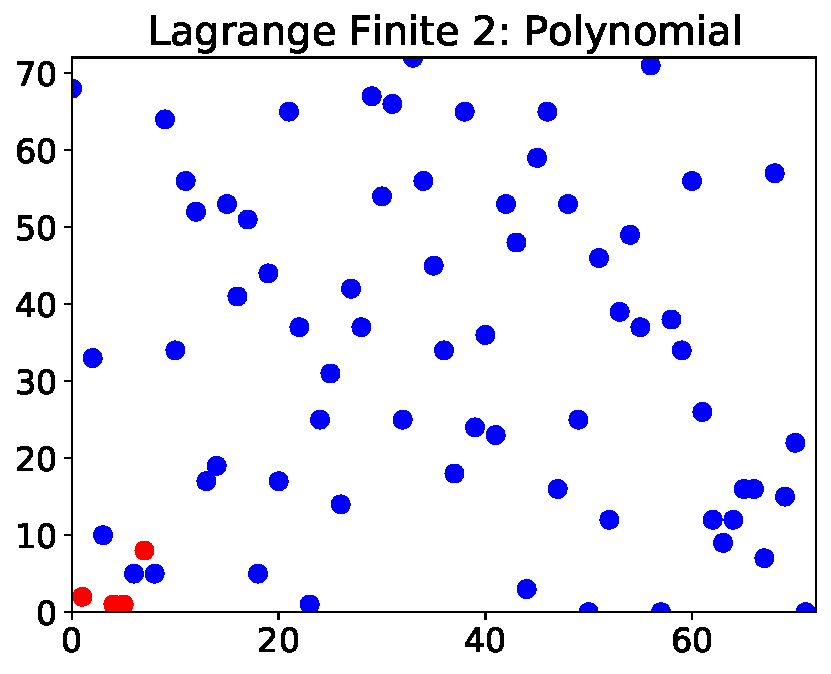
\includegraphics[width=\textwidth]{plots/lagrange/lagrange_finite_poly_2.pdf}
    \caption{Lagrange interpolation polynomial}
    \label{fig:lagrange_finite_poly_2}
    \end{subfigure}
    \caption[Data points and Lagrange Interpolation over finite fields 2]{Here
        are data points and Lagrange interpolating polynomial
        for Example~\ref{example:math_lagrange_finite_2}.
        This example uses the \gls{finite field} $\F_{73}$.}
\end{figure}



In this case, we have the interpolating polynomial

\begin{equation}
    L(x) = 60x^{3} + 51x^{2} + 42x + 68.
\end{equation}

\noindent
The data points with this polynomial can be found in
Figure~\ref{fig:lagrange_finite_poly_2}.
We see that

\begin{align}
    L(1) &= 2 \nonumber\\
    L(4) &= 1 \nonumber\\
    L(5) &= 1 \nonumber\\
    L(7) &= 8.
\end{align}
\end{example}

\subsection{Further Generalizations of Lagrange Interpolation}

It is possible to generalize \gls{lagrange interpolation} more.
In particular, by looking at Eq.~\eqref{eq:math_lagrange_def},
we see that all that is required of the data
$\braces{\parens{x_{i},y_{i}}}_{i=1}^{n}$
is that $\braces{x_{i}}$ must be elements of a \gls{field} $\F$
and $\braces{y_{i}}$ must be elements where it makes sense to perform
multiplication by $\F$.
Although this may appear to be an unnecessary generalization,
this will be used when computing threshold digital signatures
in Chapter~\ref{sec:ss_threshold};
in that setting, we are essentially interpolating over \gls{group} elements
parameterized by elements in a \gls{finite field}.
